\documentclass[10pt]{article}
\usepackage[a4paper,margin=17mm]{geometry}\usepackage[T1]{fontenc}
\usepackage{lmodern,amsmath,amssymb,graphicx,booktabs,hyperref}
\setlength{\parindent}{0pt}\setlength{\parskip}{5pt}\sloppy\setlength{\emergencystretch}{3em}
\begin{document}
\begin{center}{\Large Explicit F13 rational-point dual and subgroup inverse}\\2026-10-29; PR2381; cm8-dual-20261029\end{center}
\textbf{Verified finite result.} Independent C++ and Rust arithmetic check all14
source and14 target rational points,196 addition pairs in each direction,
both compositions equal to doubling, and all7 odd-subgroup inverses. Seven
valid target points not killed by7 are excluded from the inverse domain.
No invalid-curve experiment or generic geometric-duality claim is made.

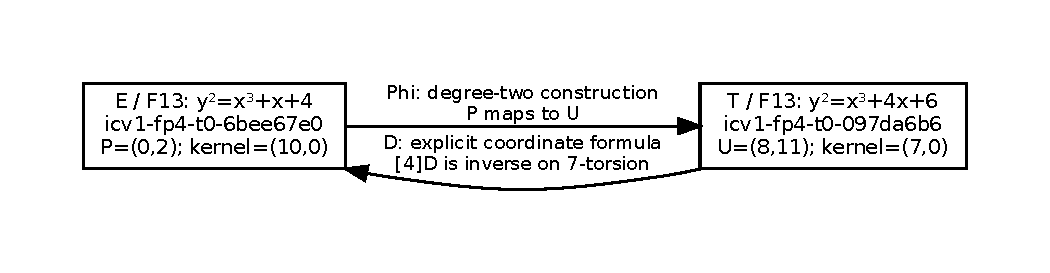
\includegraphics[width=\linewidth]{bridge.pdf}

The historical identity bindings above are missing from the merged active
registry; this does not install or validate a combined catalog. Both curves
are nonsingular. Put $v=12x-6$ on T. The new actual point function is
\[
 D(x,y)=\left(10(v+5+8/v)+10,\;12y(1-8/v^2)\right),
 \qquad I(R)=[4]D(R).
\]
Infinity and the rational kernel $(7,0)$ map to infinity. The forward map is
$\Phi(x,y)=(12(x+2/(x-10)),8y(1-2/(x-10)^2))$, with source kernel $(10,0)$.
Native and kernel-checked finite results give $D\Phi=[2]$, $\Phi D=[2]$ and
$I\Phi(Q)=Q$, $\Phi I(R)=R$ when the respective point is killed by7.
This removes enumeration from the specified public-base inverse computation;
public fixture/base construction and the rest of setup remain separate.

\textbf{Full S3 preservation.} Both native attempts execute the frozen12 arms and
72 separate nonidentity main-source recoveries. Every arm/index byte equals the
reference and original CM8 record: roots, witnesses, ordered signs/lifts,
useful rows/ranks, original/reduced degree, setup logs and source scalars.
The unchanged independent Rust S3 auditor checks both streams. All nine altered,
rehashed controls reject101 with no receipt;22 backend tests pass. The two
runs differ only in source provenance and a corrected receipt-key label;
all26 reference/candidate arm/index files match exactly, and all non-source
fields of dual.json match. Earlier mislabelled receipt is retained.

\textbf{Formal scope.} New CM8Dual.lean has21 named theorems /25 audited declarations,
zero failing or extra trusted/native axioms under the unmodified scoped gate.
Only propext, Classical.choice and Quot.sound occur. Actual Mathlib E/T point
maps use coordinate formulas, not logarithm tables. Exhaustive coordinate
coverage proves that the finite proof tables include every rational point;
then both full addition/composition statements follow. A general additive-map
lemma explicitly assumes $D(FQ)=2Q$, $2c=r+1$ and $rQ=0$, and proves
$cD(FQ)=Q$. The source-scalar theorem exposes annihilators for both unknown Q
and generator P. Its actual F13 instance accepts arbitrary natural scalars,
not only supplied generator-index labels. Geometric duality over extensions
or arbitrary fields is not inferred from finite F13 points.

Lean4.34.1, Mathlib \path{d13f23b723b8a846827a245b89c10fc7d3f11612}.
The first proof build failed at the final coercion simplification; exact source
and logs are retained. An explicit reduction fixes the same statement. Old
projects and17 polynomial certificates remain unchanged. The existing universal
translated-construction IDC1h45f7f67f60c827c3 is replayed; it certifies polynomial
arithmetic, not the whole dual/group claim. The new finite point proofs are
separate. No fresh combined count over historical projects is claimed.
\newpage
\begin{center}{\Large Request comparison, controls and remaining objective}\end{center}
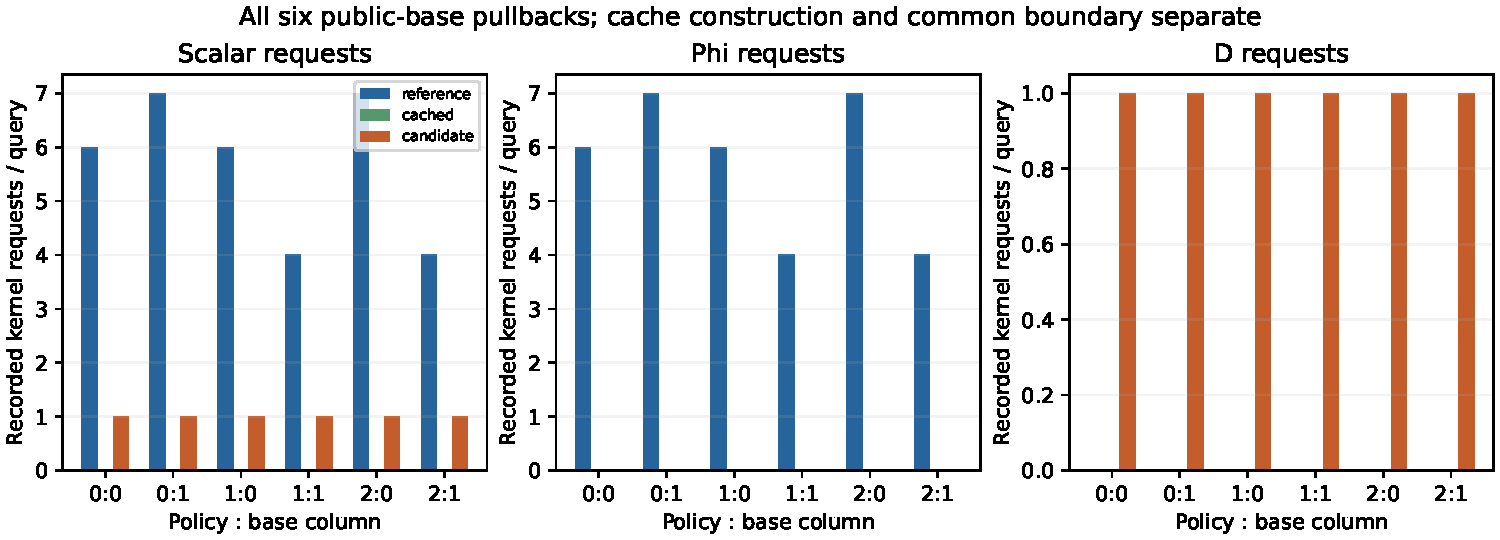
\includegraphics[width=\linewidth]{requests.pdf}
\textbf{Recorded requests.} The declared cached reference builds seven public
images once (7scalar and7Phi requests), then performs one lookup per query.
Each route additionally executes the same boundary:2scalar7 checks,1Phi
verification,2curve checks,3group comparisons. These are differently weighted
and sometimes nested requests, not time or total cost. The declared cache is
not a strongest optimized enumeration implementation. Field arithmetic,
internal scalar work, memory, lookup engineering and audit remain unpriced.

\begin{center}\begin{tabular}{lll}\toprule
Target base point & D(target) & [4]D(target) = reference inverse\\\midrule
$(6,5)$ & $(7,9)$ & $(9,1)$\\
$(8,2)$ & $(9,1)$ & $(0,11)$\\
$(11,4)$ & $(0,11)$ & $(7,9)$\\\bottomrule\end{tabular}\end{center}
Each appears twice in the six policy/column entries. The reference kernel uses
6,7,6,4,7,4 scalar/Phi/comparison requests respectively; the direct kernel uses
one D and one scalar4 request each. These counts do not establish a speed ratio.

\textbf{Yield and degree unchanged.} The earlier fixed-target CM8 comparison keeps
3of54 reduced joint gains and0original, with all four matched degree differences
favoring the source. The preceding uniform96arm/896target/210policy study keeps
0joint gains in both input forms. No new useful-yield, intrinsic regularity,
F4/F5 or calibrated complete-work advantage is claimed by an inverse change.
The original objective remains open.

\textbf{Execution flow.} One fixed native contract, two executed full attempts,
both completed, none interrupted/excluded/resumed. Attempt02 follows a frozen
metadata correction: ``nontorsion'' was a misleading receipt key because all
finite group points are torsion; the correct category is not killed by7.
The old successful source/output remains. The failed compiler adapter and
proof build are preparation/formal failures, not hidden successful runs.
Each correction was committed before affected replay; every source hash is bound.
The exact legacy Markdown protocol was committed before data; a later structured
export is metadata, not a retroactively preregistered JSON protocol or canonical
protocol-checker approval.

\textbf{Validation and holds.} Native full replay, nine corruptions, existing
certificate17, scoped Lean gate and backend tests pass. Root library validation
is separately recorded and must not be inferred green. Active1921-model
registration/catalog, naming, full library, Conductor (127/no lease), exact-head
CI/review/integration and broader completion gates remain. No paid resource or
arbitrary assets upload. Approved official branch checkpoints succeeded.
Native/proof caps600sec, science envelope18:47--19:47UTC, two local workers;
no native cap hit. No wall-time, GAE/S/rho/external-fastest/leaderboard promotion.

\textbf{Sources and reproduction.} Frozen CM8 forward source/independent audit,
CM8Transfer.lean, explicit-dual card and new preregistered protocol; known
isogeny-transfer/presentation-invariance atlas leads, no invention claim.
Run \path{run-cm8-dual.sh} with a fresh outside directory after the official
current checkpoint gate. Native records, complete raw restore, proofs and
source versions are linked from the study README. All older frozen evidence
and both catalog provenance anchors remain. Next work needs actual useful-yield/
relevant-degree evidence on a surviving encoding, plus complete main-DLP work;
a verified inverse alone does not supply it.

\end{document}
